\documentclass{report}


\usepackage[T1]{fontenc}
\usepackage[utf8]{inputenc}
\usepackage{amsmath}


\usepackage{enumerate}
\usepackage{trfsigns}
\usepackage{graphicx}
\usepackage{fancyhdr}
\usepackage{lettrine}
\usepackage{hyperref}
\usepackage{subcaption}
\usepackage{tikz}
\usepackage{cite}
\usepackage{listings}
\usepackage[nottoc, numbib]{tocbibind}
\usepackage[ngerman]{babel}
\usepackage[Glenn]{fncychap}
\usepackage{trfsigns}
\usepackage{parskip}
\usepackage{microtype}


\usetikzlibrary{shapes}
    \usetikzlibrary{arrows}
    \usetikzlibrary{arrows.meta,topaths}
    \usetikzlibrary{bending}
    \usetikzlibrary{calc}
\title{Elektrotechnik 1 Praktikum 1}


\usepackage[
  includehead,
  headheight = 17mm,
  footskip = \dimexpr\headsep+\ht\strutbox\relax,
  tmargin = 0mm,
  bmargin = \dimexpr17mm+2\ht\strutbox\relax,
]{geometry}

\usepackage{anyfontsize}
\usepackage{float}
\usepackage{xcolor}

\definecolor{DarkGreenBlue}{HTML}{264653}
\definecolor{LightGreenBlue}{HTML}{2A9D8F}
\definecolor{LightOrange}{HTML}{E9C46A}
\definecolor{DarkOrange}{HTML}{F4A261}
\definecolor{RedOrange}{HTML}{E76F51}
\definecolor{BrightRed}{HTML}{D62828}
\definecolor{DeepBlue}{HTML}{003049}

\lstdefinestyle{code}{
    backgroundcolor=\color{backcolour},
    commentstyle=\color{codegreen},
    keywordstyle=\color{magenta},
    numberstyle=\tiny\color{codegray},
    stringstyle=\color{codepurple},
    basicstyle=\ttfamily\footnotesize,
    breakatwhitespace=false,
    breaklines=true,
    captionpos=b,
    keepspaces=true,
    numbers=left,
    numbersep=5pt,
    showspaces=false,
    showstringspaces=false,
    showtabs=false,
    tabsize=2
}

\definecolor{codegreen}{rgb}{0,0.6,0}
\definecolor{codegray}{rgb}{0.5,0.5,0.5}
\definecolor{codepurple}{rgb}{0.502,0.502,0.0}
\definecolor{backcolour}{rgb}{0.95,0.95,0.95}

\pagestyle{fancy}
\fancyhead[L]{\leftmark}
\fancyhead[R]{}
\fancyfoot[L]{}
\fancyfoot[C]{\thepage}
\fancyfoot[R]{\includegraphics[scale=0.2]{../assets/images/haw.jpg}}
\renewcommand\headrulewidth{0.5pt}


\begin{document}


\thispagestyle{empty}
\begin{tikzpicture}[overlay,remember picture]
  \thispagestyle{empty}
  \fill[black!2] (current page.south west) rectangle (current page.north east);

  \begin{scope}[transform canvas ={rotate around ={45:($(current page.north west)+(-.5,-6)$)}}]

    \shade[rounded corners=18pt, left color=DarkGreenBlue, right color=LightGreenBlue] ($(current page.north west)+(-.5,-6)$) rectangle ++(9,1.5);

  \end{scope}

  \begin{scope}[transform canvas ={rotate around ={45:($(current page.north west)+(.5,-10)$)}}]

    \shade[rounded corners=18pt, left color=LightOrange,right color=DarkOrange] ($(current page.north west)+(0.5,-10)$) rectangle ++(15,1.5);

  \end{scope}

  \begin{scope}[transform canvas ={rotate around ={45:($(current page.north west)+(0.5,-10)$)}}]

    \shade[rounded corners=8pt, right color=DarkOrange, left color=LightOrange] ($(current page.north west)+(1.5,-9.55)$) rectangle ++(7,.6);

  \end{scope}

  \begin{scope}[transform canvas ={rotate around ={45:($(current page.north)+(-1.5,-3)$)}}]

    \shade[rounded corners=12pt, left color=DeepBlue!80, right color=DeepBlue!60] ($(current page.north)+(-1.5,-3)$) rectangle ++(9,0.8);

  \end{scope}

  \begin{scope}[transform canvas ={rotate around ={45:($(current page.north)+(-3,-8)$)}}]

    \shade[rounded corners=28pt, left color=BrightRed, right color=BrightRed!80] ($(current page.north)+(-3,-8)$) rectangle ++(15,1.8);

  \end{scope}

  \begin{scope}[transform canvas ={rotate around ={45:($(current page.north west)+(4,-15.5)$)}}]

    \shade[rounded corners=25pt, left color=RedOrange, right color=DarkOrange] ($(current page.north west)+(4,-15.5)$) rectangle ++(30,1.8);

  \end{scope}

  \begin{scope}[transform canvas ={rotate around ={45:($(current page.north west)+(13,-10)$)}},]

    \shade[rounded corners=22pt, left color=DeepBlue,right color=DarkGreenBlue] ($(current page.north west)+(13,-10)$) rectangle ++(15,1.5);

  \end{scope}

  \begin{scope}[transform canvas ={rotate around ={45:($(current page.north west)+(18,-8)$)}},]

    \shade[rounded corners=8pt, left color=DarkOrange] ($(current page.north west)+(18,-8)$) rectangle ++(15,0.6);

  \end{scope}

  \begin{scope}[transform canvas ={rotate around ={45:($(current page.north west)+(19,-5.65)$)}},]

    \shade[rounded corners=12pt, left color=RedOrange] ($(current page.north west)+(19,-5.65)$) rectangle ++(15,0.8);

  \end{scope}

  \begin{scope}[transform canvas ={rotate around ={45:($(current page.north west)+(20,-9)$)}}]

    \shade[rounded corners=20pt, left color=BrightRed, right color=BrightRed!80] ($(current page.north west)+(20,-9)$) rectangle ++(14,1.2);

  \end{scope}

  \draw[ultra thick,gray] ($(current page.center)+(5,2)$) -- ++(0,-3cm) node[midway,left=0.25cm,text width=5cm,align=right,black!75]{{\fontsize{25}{30} \selectfont 
\includegraphics[width=\textwidth]{./assets/img/HAW_logo.png}}} node[midway,right=0.25cm,text width=6cm,align=left,orange]{{\fontsize{70}{86} \selectfont 2023}};

  \node at ($(current page.center)+(0,-4)$) {{\fontsize{40}{72} \selectfont Leistungselektronik}};

  \node[text width=8cm,align=center] at ($(current page.center)+(0,-6.5)$) {{\fontsize{16}{20} \selectfont \textcolor{orange}{ \bf \today}} \\[3pt] Steffen Reimers 2540209\\[3pt] PF: Emily Antosch 2519935 \\[3pt] Timo Türk 2545824\\[3pt]};

\end{tikzpicture}

\newpage

\tableofcontents

\listoffigures

\newpage
\chapter{Reglersynthese - Praktikum 1}
\section{Einleitung}

In diesem Praktikum geht es um die Einführung der Messwertaufnahme im Reglersynthese-Labor. Dabei wird neben dem Berechnen des RC-Glieds mit Messwiderstand auch eine Messwertaufnahme mittels Matlab Desktop Live betrachtet. Kennwerte einer Ladungskurve werden mit den Matlab Bordmitteln(Curve Fitter) errechnet und zum Schluss mit der Berechnung verglichen.


\section{Vorbereitung}
In der Vorbereitung soll nun eine mathematische Betrachtung für den Versuch errechnet werden:

\begin{equation}
  u_c(t) + R\cdot (i_{rm}(t)+i_c(t)) - u_e(t) = 0 
  \label{eq:masche}
\end{equation}

Nun ersetzen werden die Ströme in der Gleichung ersetzt:

\begin{equation}
  u_c(t) + R\cdot (\frac{u_c(t)}{R_M}+\frac{du_c}{dt} C) = u_e(t)  
  \label{eq:ersetz_i}
\end{equation}

Nun transformieren wir die Gleichung~\ref{eq:ersetz_i}:

\begin{equation}
  u_e(t) \laplace U_e(s) = U_c(s) \cdot \frac{R_M+R}{R_M} + RCs\cdot U_c(s)
  \label{eq:laplace}
\end{equation}

Nach weiterem Umformen ergibt sich dann eine Übertragungsfunktion von: 

\begin{equation}
  \frac{U_c(s)}{U_e(s)} = \displaystyle\frac{\frac{R_M}{R_M+R}}{1+\frac{R\cdot R_M}{R_M + R}\cdot C \cdot s} = \frac{k_p}{1+R_gCs} 
  \label{eq:ueber}
\end{equation}

Zum Schluss soll nun noch die Sprungantwort berechnet werden. Dazu wird die Übertragungsfunktion invers transformiert und der Eingangssprung auf das System gegeben:

\begin{equation}
  U_c(s) = \frac{1}{s}\cdot\frac{k_p}{1+R_gCs}\\
  U_c(s)  \Laplace  u_c(t) = \sigma(t) \cdot k_p(1-e^{-\frac{t}{R_gC}})
  \label{eq:step_resp}
\end{equation}


\section{Durchführung}

Nun wird das System im Labor aufgebaut und durch das Matlab Realtime Desktop System gemessen. Zunächst wird ein Offset-Ausgleich an den Eingängen des System gemacht. Im Anschluss wird ein RC-Glied wie in der Aufgabenstellung zu sehen angeschlossen. Zur Messung wird ein Sprung von $0V$ auf $5V$ und wieder auf $0V$ aufgenommen und dann untersucht. Die Betriebsmittel haben einen Wert von $C = 1nF$ und $R = 390k\Omega$.

\section{Beobachtung}

Die Messung ergibt die Trace, die in Abbildung~\ref{fig:step_resp} zu sehen ist. Zu erkennen ist deutlich, dass ein $k_p < 1$ besteht, da die 5V, die maximal erreichbar wären, deutlich verfehlt werden. 

\begin{figure}[h]
  \begin{center}
    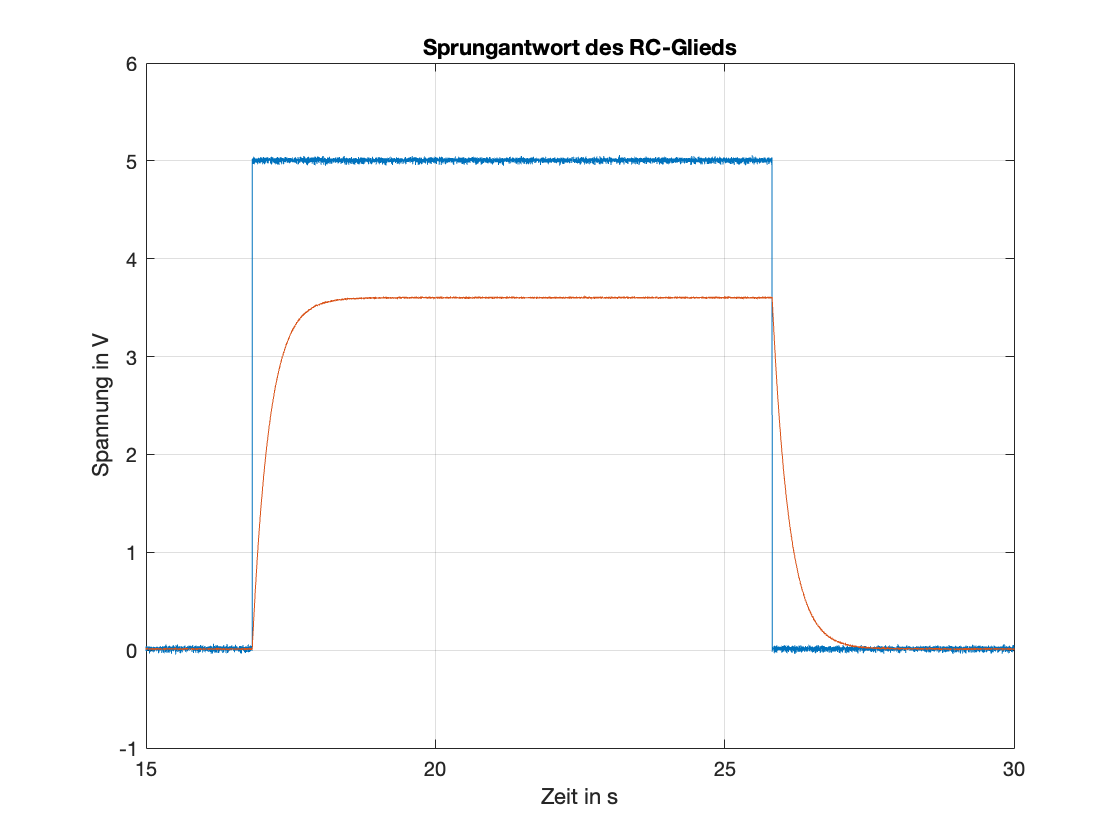
\includegraphics[width=0.95\textwidth]{assets/img/step_response.png}
  \end{center}
  \caption{Die Sprungantwort des Systems}
  \label{fig:step_resp}
\end{figure}

Mittels des Tools "Curve Fitter" wird nun die Kurve mittels der in der Vorbereitung berechneten Formel angenähert. Das Tool gibt dann die Parameter aus, mit denen dann die Betriebsmittel rückwirkend berechnet werden können.

\section{Auswertung}

Aus dem Fitting kann ein Wert für $k_p = 0.718$ und für $T = 0.2918s$ bestimmt werden. Aus der Vorbereitung kann nun ein Wert für den Eingangswiderstand $R_M$ berechnet werden:

\begin{equation}
  k_p = \frac{R_M}{R_M + R}\\
  R_M = \frac{-k_p\cdot R}{k_p-1} = \frac{-0,718 \cdot 390k\Omega}{0,718-1} = 
  \label{eq:rm}
\end{equation}
Nun kann auch mit der Zeitkonstante noch die Angabe des Kondensator von $C = 1nF$ überprüft werden:

\begin{equation}
  T = \frac{}{} 
  \label{eq:kondensator_ueberpruefen}
\end{equation}
\end{document}
